
% Define which ratio you want to use 
%         43 to have a 4:3, 
%         169 to have 16:9.

\def\currentAspect{169}

\documentclass[t,aspectratio=\currentAspect]{beamer}


\definecolor{c1}{rgb}{0,0.4470,0.7410}
\definecolor{c2}{rgb}{0.8500,0.3250,0.0980}
\definecolor{c3}{rgb}{0.9290,0.6940,0.1250}
\definecolor{c4}{rgb}{0.4940,0.1840,0.5560}
\definecolor{c5}{rgb}{0.4660,0.6740,0.1880}
\definecolor{c6}{rgb}{0.3010,0.7450,0.9330}
\definecolor{c7}{rgb}{0.6350,0.0780,0.1840}
\definecolor{c8}{rgb}{0,0.4325,0.1746}

\def\oldAspect{43}
\def\newAspect{169}

\setbeamercolor{block title}{fg=c1,bg=white} % Colors of the block titles
\setbeamercolor{block body}{fg=black,bg=white} % Colors of the body of blocks
\setbeamercolor{block alerted title}{fg=white,bg=c1} % Colors of the highlighted block titles
\setbeamercolor{block alerted body}{fg=black,bg=c1!10} % Colors of the body of highlighted blocks
\setbeamercolor{frametitle}{fg=c1,bg=white} % Colors of the block titles

\setbeamersize{text margin left=5mm,text margin right=5mm} 
\setbeamertemplate{footline}[frame number]

\usepackage{tcolorbox}
\RequirePackage[english]{babel}
\usepackage[linesnumbered,ruled,vlined]{algorithm2e}
\usepackage{mathrsfs,amsmath}
\usepackage{listings}
\usepackage{linehighlight}

\usepackage{pgfgantt}
\usepackage{pgfplots}
\usepackage{tikz}
\usetikzlibrary{intersections}
\usetikzlibrary{shapes}
\usetikzlibrary{chains}
\usetikzlibrary{arrows,positioning,calc}
\usetikzlibrary{decorations.markings}
\usetikzlibrary{patterns}
\usetikzlibrary{shapes.geometric}
\usetikzlibrary{matrix}
\usepackage[outline]{contour}
\usetikzlibrary{positioning}
\usetikzlibrary{trees}
\usetikzlibrary{patterns}
\usetikzlibrary{backgrounds}
\usetikzlibrary{arrows,shapes}
\usetikzlibrary{chains}
\usetikzlibrary{calc}
\usetikzlibrary{matrix}
\usetikzlibrary{decorations.pathreplacing}
\usetikzlibrary{decorations}
\usepackage{tikz-3dplot}
\usepgfplotslibrary{groupplots}
\usepackage{subcaption}
\usepgfplotslibrary{clickable}
\newtcolorbox{mybox}[1][]
{
  colframe = c1,
  sharpish corners,
  colback  = white
}

\setbeamertemplate{frametitle}{%
    \usebeamerfont{frametitle}\insertframetitle%
    \vphantom{g}% To avoid fluctuations per frame
    %\hrule% Uncomment to see desic2 effect, without a full-width hrule
    \par\hspace*{-\dimexpr0.5\paperwidth-0.5\textwidth}  \rule[0.5\baselineskip]{\paperwidth}{1.4pt}
    \par\vspace*{-\baselineskip}% <-- reduce vertical space after rule
}

\setbeamertemplate{itemize item}{\color{c1}$\blacktriangleright$}
\setbeamertemplate{itemize subitem}{\color{c2}$\blacktriangleright$}

\setbeamercolor{caption name}{fg=c1}

\newcommand{\argmin}{\operatornamewithlimits{arg\,min}}


%\setbeamertemplate{section in toc}[square unnumbered]
\setbeamercolor{section in toc}{fg=black}

\lstdefinelanguage
   [x64]{Assembler}     % add a "x64" dialect of Assembler
   [x86masm]{Assembler} % based on the "x86masm" dialect
   % with these extra keywords:
   {morekeywords={CDQE,CQO,CMPSQ,CMPXCHG16B,JRCXZ,LODSQ,MOVSXD, %
                  POPFQ,PUSHFQ,SCASQ,STOSQ,IRETQ,RDTSCP,SWAPGS, %
                  rax,rdx,rcx,rbx,rsi,rdi,rsp,rbp, vpxorq,   xor,  nopl,  vmovupsz ,  leal, vmovupsz, vcmppdz, vdivpdz, vmovupdz,%
                  r8,r8d,r8w,r8b,r9,r9d,r9w,r9b, %
                  r10,r10d,r10w,r10b,r11,r11d,r11w,r11b,zmm0,zmm1,zmm2,k1,k2, %
                  r12,r12d,r12w,r12b,r13,r13d,r13w,r13b, %
                  r14,r14d,r14w,r14b,r15,r15d,r15w,r15b}} % etc.


\definecolor{codehighlight}{rgb}{0.8500,0.3250,0.0980}
\definecolor{codebackground}{rgb}{1,1,1}

\newcommand{\gwidthd}{0.975\linewidth}
\newcommand{\gheightd}{0.6\linewidth}  
\newcommand{\gheightdd}{0.4\linewidth}  

\newcommand{\figurewidth}{0.9\linewidth}  
\newcommand{\figureheight}{0.9\textheight}  
\newcommand{\figureheightt}{0.7\linewidth}  

\newcommand{\Mod}[1]{\ (\mathrm{mod}\ #1)}


\usepackage{courier}


\pgfplotsset{
    clickable coords = {(xy)}, % activates a snap-to-nearest feature
    annot/snap dist=20,
    /pgfplots/annot/js fillColor={["RGB",0,0.4470,0.7410]},
    /pgfplots/annot/point format/.initial={(\%.1f, \%.1f)},
    every semilogy axis/.append style={/pgfplots/annot/point format={(\%.1f,\%.1e)}},
    every semilogx axis/.append style={/pgfplots/annot/point format={(\%.1e,\%.1f)}},
    every loglog axis/.append style={/pgfplots/annot/point format={(\%.1e,\%.1e)}},
    %clickable coords size = {7,3}, % size in characters for the snapping pop ups
    %annot/popup size generic = {8,4}, % size in characters  for the rest
}

\begin{document}


\AtBeginSection[]
{
   \begin{frame}[plain,noframenumbering]
        \frametitle{Table of contents}
        \tableofcontents[currentsection]
   \end{frame}
}


\beamertemplatenavigationsymbolsempty
\begin{frame}[plain,noframenumbering]

\vspace{10pt}

\begin{mybox}
\begin{center}
\parbox{.06\textwidth}{
\includegraphics[height=12pt]{logos/FNRS.eps}}
\parbox{.13\textwidth}{
\includegraphics[height=18pt]{logos/uLIEGE.eps}}
\parbox{.54\textwidth}{\centering \scriptsize Very long title}
\parbox{.13\textwidth}{
\includegraphics[height=18pt]{logos/uLIEGE.eps}}
\parbox{.06\textwidth}{
\includegraphics[height=12pt]{logos/FNRS.eps}}
{ \tiny \underline{Author 1}, Author 2, Author 3}
\end{center}
\end{mybox}

\vspace{-10pt}
\begin{center}
\resizebox{1.\textwidth}{!}{%
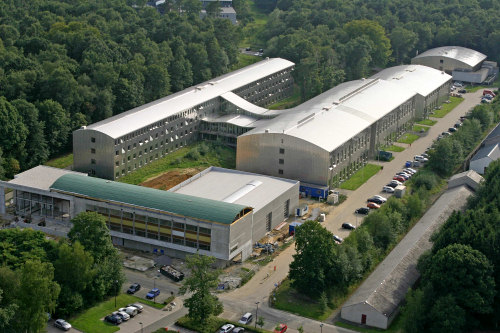
\includegraphics[height=5cm]{buildings/ulg.jpg}%
\quad
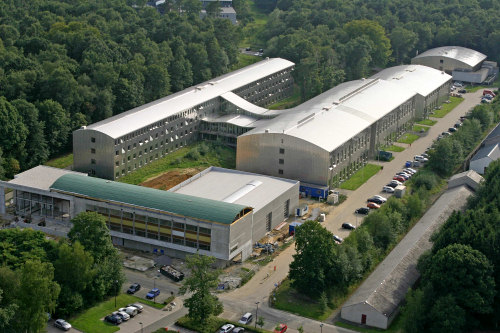
\includegraphics[height=5cm]{buildings/ulg.jpg}
\quad
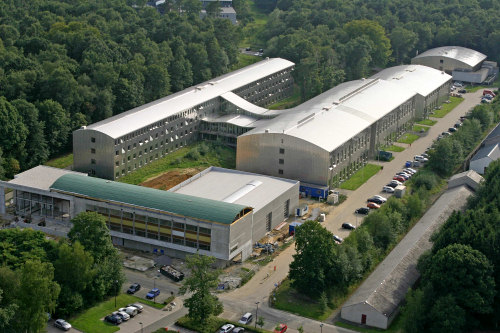
\includegraphics[height=5cm]{buildings/ulg.jpg}%
}
\end{center}

\begin{center}
Where do I present?\\
\today.
\end{center}
\end{frame}



% Example to show how to test whether the pdf is built with 4:3 or 16:9 ratio:
\ifx\currentAspect\oldAspect
	\def\sometext{The code has been built with the ratio for old screens 4:3}
\else
	\def\sometext{The code has been built with the ratio for new screens 16:9}
\fi



\begin{frame}{Slide }
\begin{itemize}
\setlength\itemsep{\fill}
\item \sometext,
\item Bullet 2,
\item Bullet 3,
\item Bullet 4.
\end{itemize}
\end{frame}

\end{document}